\chapter{Experimentos y resultados}
\label{chapter:experimentos_y_resultados}
En este capítulo vamos a comentar los experimentos realizados para cada objetivo y los resultados obtenidos.

%%% SECTION
\section{Experimentos}
Los experimentos realizados en este TFM han sido modelados y ejecutados íntegramente en el entorno \textit{``Big Data"} de Databricks Community Edition, tanto para el objetivo de predecir la facturación de los clientes, como para la predicción del canal por el que se ha realizado una reclamación. Seguidamente describiremos por separado cada uno de ellos.

\subsection{Predicción de facturación electrónica de los clientes}

El conjunto de datos cargado en la plataforma contaba con 1.000.000 registros de clientes. El conjunto era mayor en un inicio, pero por restricciones de espacio en la versión gratuita de Databricks se hizo un filtrado previo.
Todos los clientes tienen informado el campo que determina si la facturación se le envía por vía correo postal o por correo electrónico, así que podemos usar todo el \textit{dataset} sin necesidad de filtros adicionales.


Tras realizar un análisis exploratorio de los datos, vemos que la cantidad de clientes que tienen un u otro estado no es proporcionado, pues es más de cinco veces mayor la cantidad de clientes que tienen facturación por correo postal de los que tienen facturación electrónica.
Esto se conoce como datos desbalanceados (\textit{``imbalanced data"} en inglés), y ocurre en los problemas de clasificación cuando en nuestros datos de entrenamiento tenemos alguna clase minoriataria. Este problema puede conllevar una bajada calidad en nuestros modelos, ya que se entrenarían con datos mayoritariamente de una clase y aprenderían más de una que de otra. Incluso pueden llegar a simplificar la clasificación determinando que la predicción siempre es de la clase mayoritaria obteniendo buenos resultados en la precisión.
Por ejemplo, en este mismo caso que estamos tratando donde una clase es cinco veces mayor que la otra la precisión de este tipo de modelo sería del 80\%.

Para tratar el problema de datos desbalanceados existen varios métodos:
\begin{itemize}
    \item Undersampling:
    
    \textit{``Undersampling"} es el proceso donde aleatoriamente se eliminan algunas de las observaciones de la clase mayoritaria hasta hacerla coincidir con el número de observaciones de la clase minoritaria.
    
    \item Oversampling:
    
    \textit{``Oversampling"} es un proceso más complejo que el anterior y se basas en generar datos sintéticos a partir de las observaciones de la clase minoritaria.
    Hay una gran variedad de métodos usados para este proceso, pero el más común es el llamado SMOTE (acrónimo en inglés de \textit{``Synthetic Minority Over-sampling Technique"}).

    \item Ensemble Classifiers:
    
    Utiliza las ventajas de hacer un ensamblado de métodos de clasificación, es decir, entrena diversos modelos y entre todos obtiene el resultado final (como un sistema democrático de votaciones) pero se asegura de tomar muestras de entrenamiento equilibradas.
    
\end{itemize}

Para prevenir que esta desproporción pueda afectar a la calidad de los modelos y dado que disponemos de un conjunto de datos todavía considerable, se decide hacer un \textit{``Undersampling"} tomando una muestra aleatoria de 150.000 registros de cada tipo y juntándolos en un nuevo \textit{dataset} de 300.000 registros en total.


\subsection{Predicción del canal por el que se ha realizado una reclamación}

Para el caso de la predicción del canal de reclamaciones y quejas no fue necesario realizar un filtrado de los datos para cargarlos en el entorno de Databricks, ya que este conjunto de datos es una división del resto de acciones de los clientes con la empresa y en total sumaba 448.589 registros.

Como sucedió en el caso anterior, la cantidad de casos de una u otra tipología es desproporcionada. Casi cuatro veces mayor son las reclamaciones realizadas por plataformas no digitales de las que sí lo son.
Igual que con el \textit{dataset} de clientes, para prevenir una pérdida en la calidad de los modelos, se tomará una muestra aleatoria de 90.000 registros de cada tipo y se juntarán en nuevo conjunto de datos de 180.000 registros en total.

%%% SECTION
\section{Resultados}

A continuación mostraremos los resultados de los modelos  para cada uno de estos objetivos, de los cinco tipos distintos de clasificación.

\subsection{Predicción de facturación electrónica de los clientes}

Como veremos a continuación en el detalle de cada modelo de predicción, los modelos han obtenido para este objetivo una buena calidad en sus predicciones, con una exactitud y un F1 en torno al 0.85 en la mayoría de ellos.

\begin{itemize}

%\begin{minipage}{\linewidth}
    \item Logistic Regression

El modelo de regresión logística ha obtenido un buena calidad como podemos ver en la siguientes gráficos y métricas.
\\

Gráficos:    
\begin{figure}[H]
\centerline{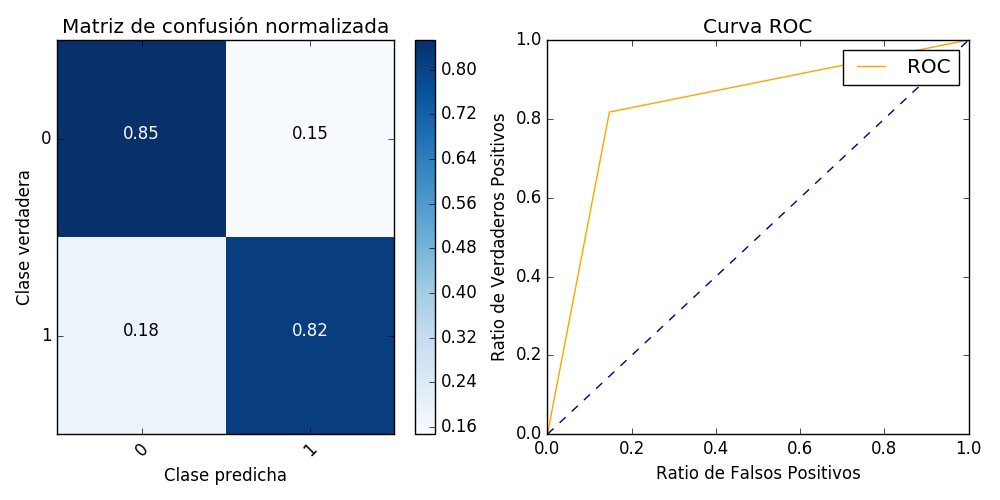
\includegraphics[width=1.0\textwidth]{TFM/figs/gra_cli_lr.png}}
\caption{Logistic Regression}
\label{fig:gra_cli_lr}
\end{figure}
Métricas:
\begin{verbatim}
Exactitud (ACC): 0.84
Error de clasificación (ERR): 0.16
Tasa de verdaderos positivos o sensibilidad (TPR | REC): 0.82
Tasa de verdaderos negativos (FPR): 0.15
Precisión (PRE)): 0.85
Especificidad(SPE): 0.85
F1: 0.83
Área bajo la curva ROC: 0.91
\end{verbatim}
%\end{minipage}

\begin{minipage}{\linewidth}
    \item Decision Tree Classifier

El Decision Tree Classifier ha obtenido uno de los peores resultados en comparación con el resto de modelos, porque ha fallado sobretodo en la tasa de verdaderos negativos (PFR).
\\

Gráficos:
\begin{figure}[H]
\centerline{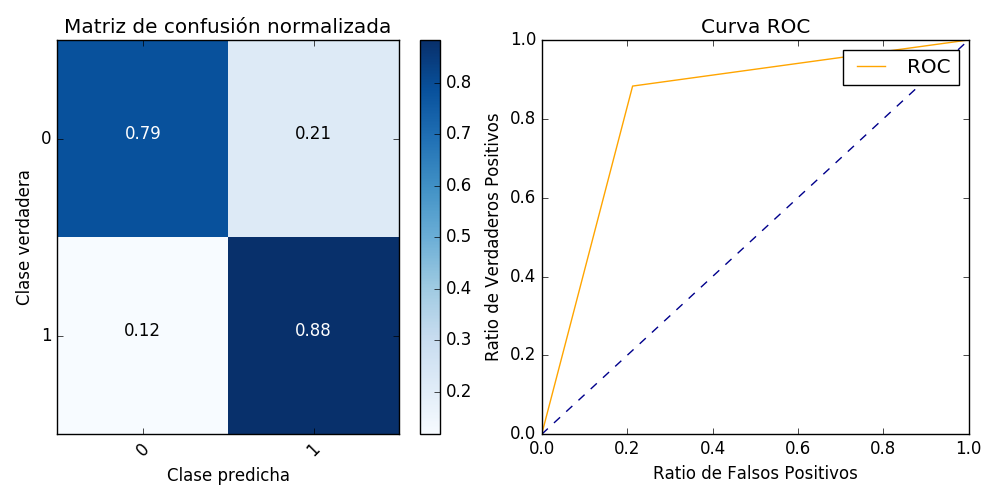
\includegraphics[width=1.0\textwidth]{TFM/figs/gra_cli_dtc.png}}
\caption{Decision Tree Classifier}
\label{fig:gra_cli_dtc}
\end{figure}
Métricas:
\begin{verbatim}
Exactitud (ACC): 0.84
Error de clasificación (ERR): 0.16
Tasa de verdaderos positivos o sensibilidad (TPR | REC): 0.88
Tasa de verdaderos negativos (FPR): 0.21
Precisión (PRE)): 0.81
Especificidad(SPE): 0.79
F1: 0.84
Área bajo la curva ROC: 0.90
\end{verbatim}
\end{minipage}

\begin{minipage}{\linewidth}
    \item Random Forest Classifier
    
El Random Forest Classifier vemos que ha fallado en lo mismo que el Decision Tree Classifier, esto puede ser explicado puesto que son de la misma familia. A continuación mostramos sus gráficos y métricas.
\\

Gráficos:
\begin{figure}[H]
\centerline{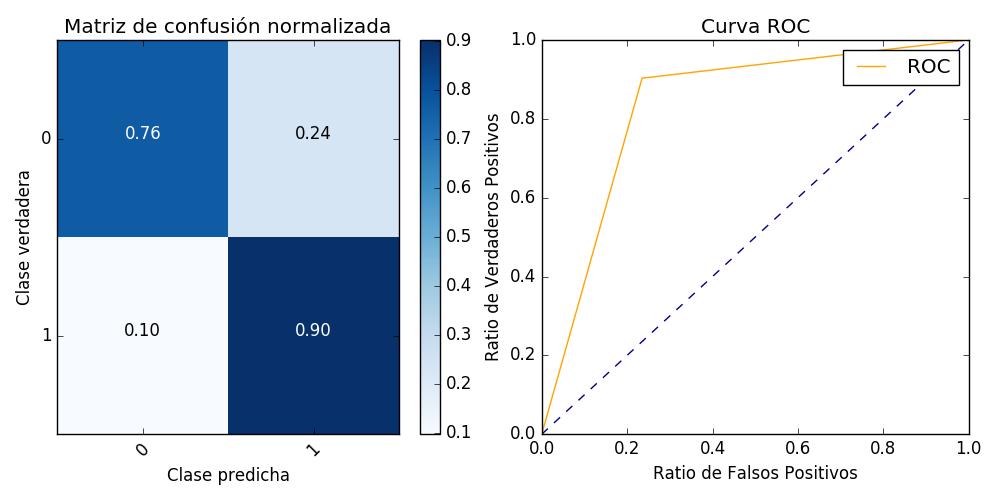
\includegraphics[width=1.0\textwidth]{TFM/figs/gra_cli_rfc.png}}
\caption{Random Forest Classifier}
\label{fig:gra_cli_rfc}
\end{figure}
Métricas:
\begin{verbatim}
Exactitud (ACC): 0.83
Error de clasificación (ERR): 0.17
Tasa de verdaderos positivos o sensibilidad (TPR | REC): 0.90
Tasa de verdaderos negativos (FPR): 0.24
Precisión (PRE): 0.79
Especificidad(SPE): 0.76
F1: 0.84
Área bajo la curva ROC: 0.91
\end{verbatim}
\end{minipage}

\begin{minipage}{\linewidth}
    \item Gradient-boosted Tree Classifier
    
El Gradient-boosted Tree Classifier ha obtenido uno de los mejores resultados, como podemos apreciar en los gráficos y métricas a continuación:
\\

Gráficos:
\begin{figure}[H]
\centerline{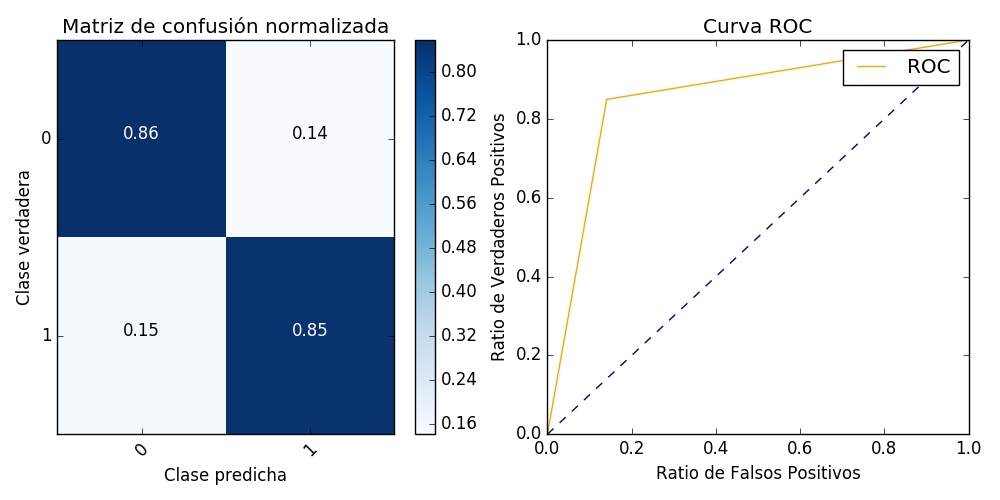
\includegraphics[width=1.0\textwidth]{TFM/figs/gra_cli_gbtc.png}}
\caption{Gradient-boosted Tree Classifier}
\label{fig:gra_cli_gbtc}
\end{figure}
Métricas:
\begin{verbatim}
Exactitud (ACC): 0.85
Error de clasificación (ERR): 0.15
Tasa de verdaderos positivos o sensibilidad (TPR | REC): 0.85
Tasa de verdaderos negativos (FPR): 0.14
Precisión (PRE): 0.86
Especificidad(SPE): 0.86
F1: 0.85
Área bajo la curva ROC: 0.93
\end{verbatim}
\end{minipage}

\begin{minipage}{\linewidth}
    \item Linear Support Vector Machine

Este modelo ha sido el que mejor calidad muestra en el objetivo de la predicción de facturación electrónica.
Como se puede observar a continuación, este modelo obtiene las mejores métricas de entre todos los modelos.
\\

Gráficos:
\begin{figure}[H]
\centerline{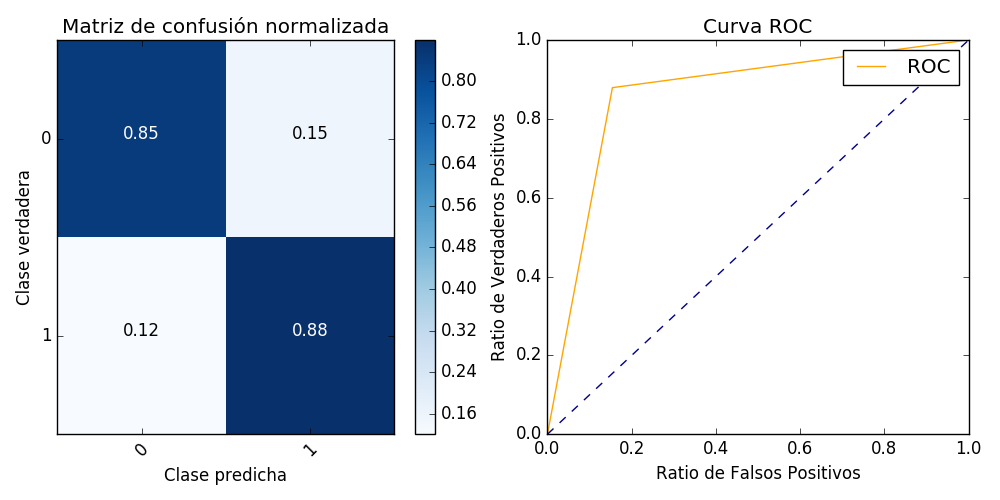
\includegraphics[width=1.0\textwidth]{TFM/figs/gra_cli_lsvm.png}}
\caption{Linear Support Vector Machine}
\label{fig:gra_cli_lsvm}
\end{figure}
Métricas:
\begin{verbatim}
Exactitud (ACC): 0.86
Error de clasificación (ERR): 0.14
Tasa de verdaderos positivos o sensibilidad (TPR | REC): 0.88
Tasa de verdaderos negativos (FPR): 0.15
Precisión (PRE)): 0.85
Especificidad(SPE): 0.85
F1: 0.86
Área bajo la curva ROC: 0.93
\end{verbatim}
\end{minipage}

\end{itemize}
\clearpage

\subsection{Predicción del canal por el que se ha realizado una reclamación}
Como veremos a continuación, los modelos de predicción del canal por el que se ha realizado una reclamación no han obtenido tan buenos resultados como los del anterior objetivo. Estos modelos han obtenido una exactitud y F1 en torno al 0.8.

\begin{itemize}

\begin{minipage}{\linewidth}
    \item Logistic Regression
    
El modelo de Logistic Regression ha obtenido una baja calidad en comparación con el resto de modelos para este objetivo, siendo su exactitud y F1 en torno a 0.75.
\\

Gráficos:    
\begin{figure}[H]
\centerline{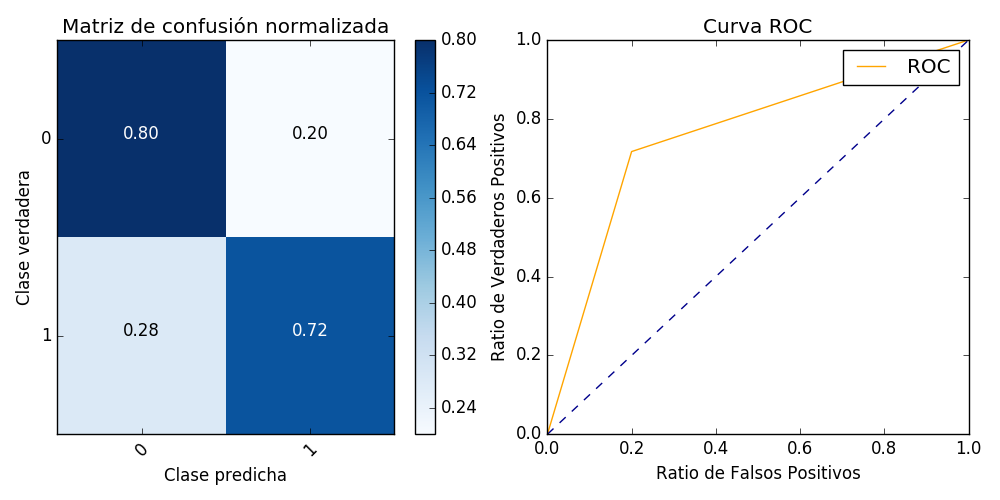
\includegraphics[width=1.0\textwidth]{TFM/figs/gra_acc_lr.png}}
\caption{Logistic Regression}
\label{fig:gra_acc_lr}
\end{figure}
Métricas:
\begin{verbatim}
Exactitud (ACC): 0.76
Error de clasificación (ERR): 0.24
Tasa de verdaderos positivos o sensibilidad (TPR | REC): 0.72
Tasa de verdaderos negativos (FPR): 0.20
Precisión (PRE)): 0.78
Especificidad(SPE): 0.80
F1: 0.75
Área bajo la curva ROC: 0.84
\end{verbatim}
\end{minipage}

\begin{minipage}{\linewidth}
    \item Decision Tree Classifier
    
El modelo Decision Tree Classifier ha obtenido uno de los mejores resultados, siendo su exactitud/F1 en torno al 0.8.
\\

Gráficos:
\begin{figure}[H]
\centerline{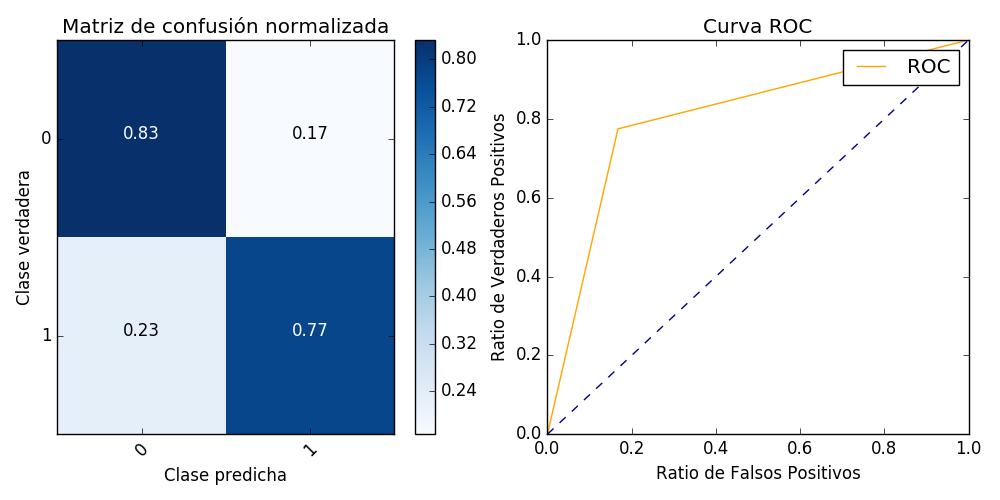
\includegraphics[width=1.0\textwidth]{TFM/figs/gra_acc_dtc.png}}
\caption{Decision Tree Classifier}
\label{fig:gra_acc_dtc}
\end{figure}
Métricas:
\begin{verbatim}
Exactitud (ACC): 0.80
Error de clasificación (ERR): 0.20
Tasa de verdaderos positivos o sensibilidad (TPR | REC): 0.77
Tasa de verdaderos negativos (FPR): 0.17
Precisión (PRE)): 0.82
Especificidad(SPE): 0.83
F1: 0.80
Área bajo la curva ROC: 0.82
\end{verbatim}
\end{minipage}

\begin{minipage}{\linewidth}
    \item Random Forest Classifier
    
El modelo Random Forest Classifier ha obtenido una buena calidad aunque un poco menor que su homólogo Decision Tree Classifier.
\\

Gráficos:
\begin{figure}[H]
\centerline{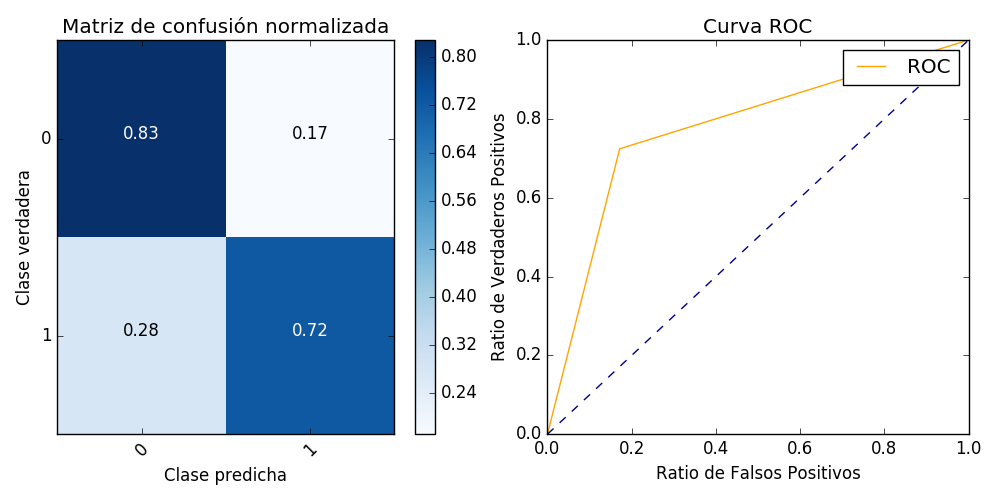
\includegraphics[width=1.0\textwidth]{TFM/figs/gra_acc_rfc.png}}
\caption{Random Forest Classifier}
\label{fig:gra_acc_rfc}
\end{figure}
Métricas:
\begin{verbatim}
Exactitud (ACC): 0.78
Error de clasificación (ERR): 0.22
Tasa de verdaderos positivos o sensibilidad (TPR | REC): 0.72
Tasa de verdaderos negativos (FPR): 0.17
Precisión (PRE)): 0.81
Especificidad(SPE): 0.83
F1: 0.76
Área bajo la curva ROC: 0.85
\end{verbatim}
\end{minipage}

\begin{minipage}{\linewidth}
    \item Gradient-boosted Tree Classifier
    
Este modelo ha sido el que mejores resultados ha conseguido en la predicción de este objetivo, siendo su exactitud/F1 de un 0.8 aproximadamente.
\\

Gráficos:
\begin{figure}[H]
\centerline{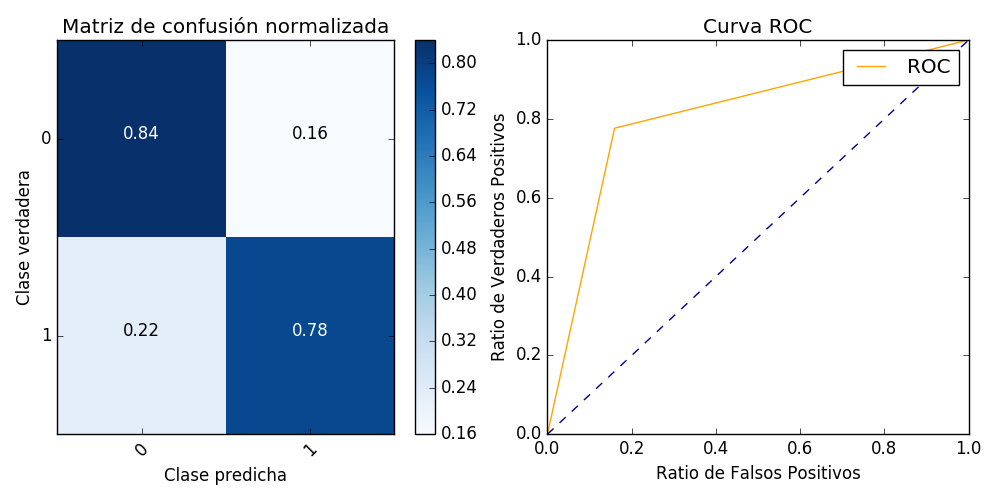
\includegraphics[width=1.0\textwidth]{TFM/figs/gra_acc_gbtc.png}}
\caption{Gradient-boosted Tree Classifier}
\label{fig:gra_acc_gbtc}
\end{figure}
Métricas:
\begin{verbatim}
Exactitud (ACC): 0.81
Error de clasificación (ERR): 0.19
Tasa de verdaderos positivos o sensibilidad (TPR | REC): 0.78
Tasa de verdaderos negativos (FPR): 0.16
Precisión (PRE)): 0.83
Especificidad(SPE): 0.84
F1: 0.80
Área bajo la curva ROC: 0.89
\end{verbatim}
\end{minipage}

\begin{minipage}{\linewidth}
    \item Linear Support Vector Machine
    
El modelo Linear Support Vector Machine ha obtenido una baja calidad en comparación a otros modelos en este mismo objetivo. 
\\

Gráficos:
\begin{figure}[H]
\centerline{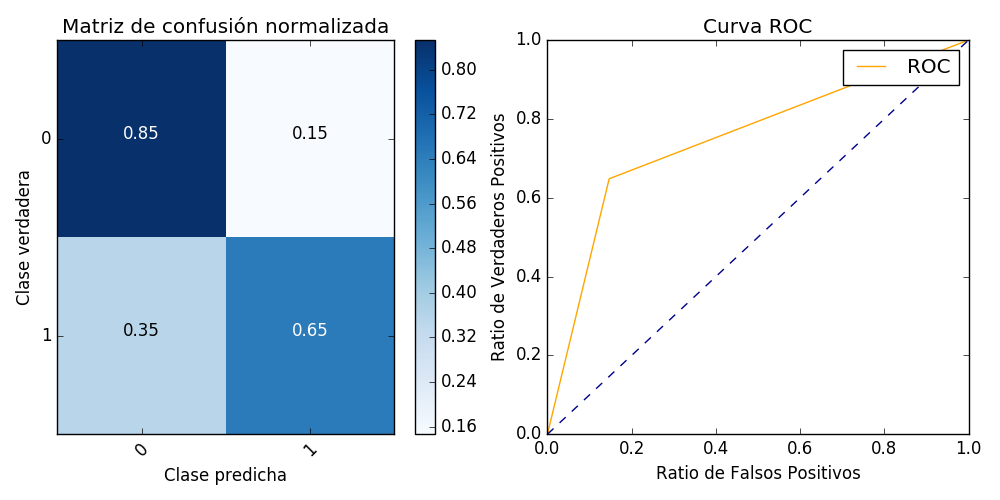
\includegraphics[width=1.0\textwidth]{TFM/figs/gra_acc_lsvm.png}}
\caption{Linear Support Vector Machine}
\label{fig:gra_acc_lsvm}
\end{figure}
Métricas:
\begin{verbatim}
Exactitud (ACC): 0.75
Error de clasificación (ERR): 0.25
Tasa de verdaderos positivos o sensibilidad (TPR | REC): 0.65
Tasa de verdaderos negativos (FPR): 0.15
Precisión (PRE)): 0.82
Especificidad(SPE): 0.85
F1: 0.72
Área bajo la curva ROC: 0.82
\end{verbatim}
\end{minipage}

\end{itemize}

